
\setcounter{section}{0}
\setcounter{figure}{0}
\graphicspath{{./figs/}{./figs/item-yanzhi/}}

\NewsTitle{Luminescent Solar Concentrator-Based Reconfigurable Photovoltaic System for EV/HEV}
\NewsAuthor{Yanzhi Wang, Caiwen Ding, Syracuse University}

Photovoltaic (PV) cells provide us a clean and quiet form of electrical energy generation, and can be an ideal power source for EVs and HEVs. In general, the onboard PV system can provide up to 20\%-30\% of propelling power for a normal EV/HEV during cruising and city driving (which takes <10kW), and perhaps more importantly, it could charge the EV/HEV battery pack during parking time to reduce the recharging requirement and mitigate the power demand from the grid.

\begin{figure}[h]
    \centering
%    \includegraphics{right}{Figure4}
    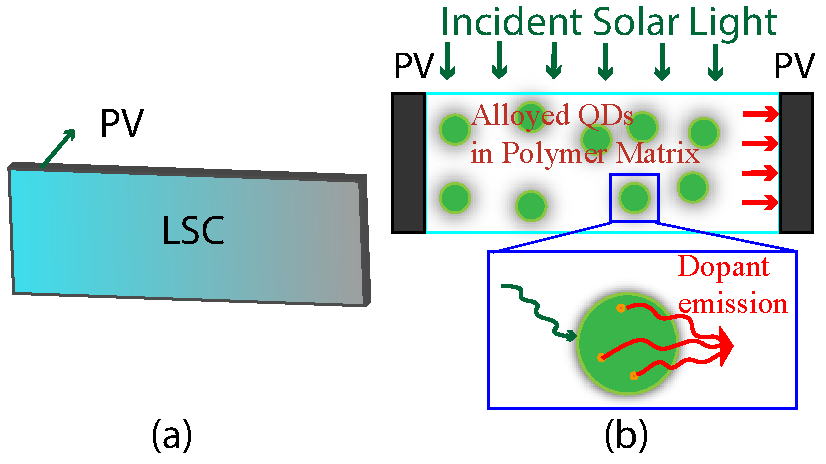
\includegraphics[width=.36\textwidth]{Figure4}
    \caption{(a) Top view and (b) vertical cross section schematic of LSC-enhanced PV cell.}
    \label{fig:1}
\end{figure}

%\begin{center}
%    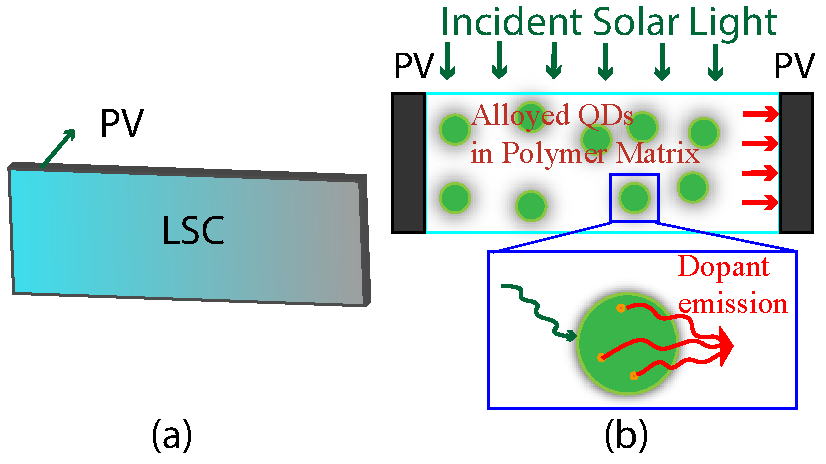
\includegraphics[width=.44\textwidth]{Figure4}
%    \caption{(a) Top view and (b) vertical cross section schematic of LSC-enhanced PV cell.}
%    \label{fig:1}
%\end{center}



\begin{figure}[h]
    \centering
%    \includegraphics{right}{Figure4}
    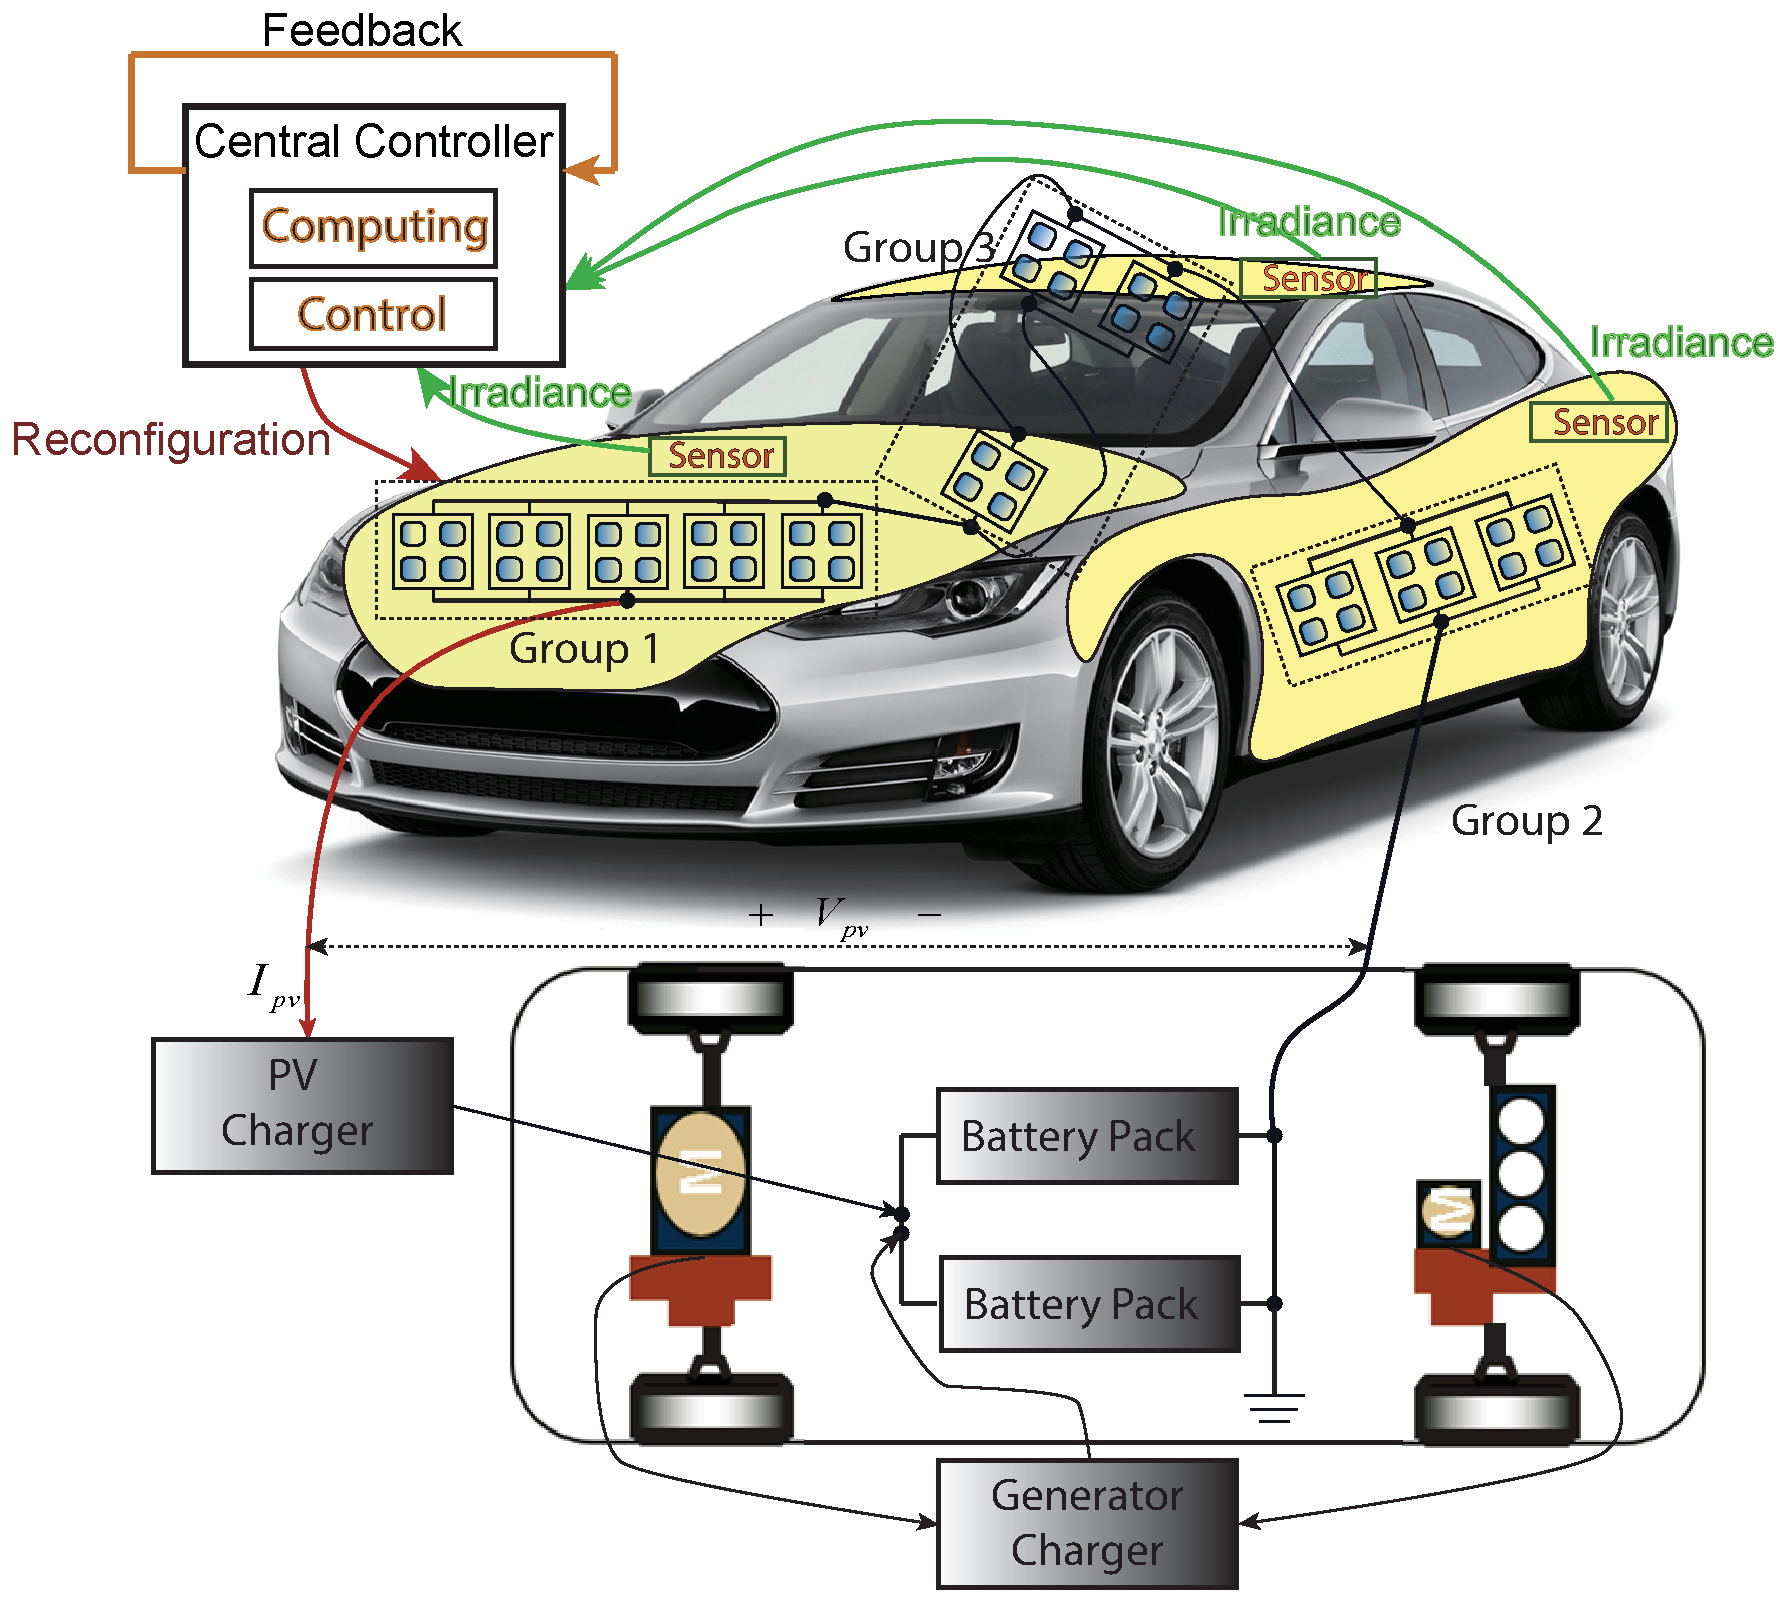
\includegraphics[width=.44\textwidth]{PV_HPEV_proposal_update}
    \caption{System diagram of an LSC-enhanced reconfigurable onboard PV
system.}
    \label{fig:2}
\end{figure}



To increase PV power generation for EV/HEV, we should enlarge onboard PV cell modules by using all possible vehicle surface areas including the rooftop, hood, trunk, and door panels. These PV cell modules are connected to the EV/HEV battery pack through one power converter. This structure is called string charger architecture, and is a practical choice for onboard PV system accounting for cost considerations and high voltage of EV/HEV battery pack~\cite{xiao2007topology,hamilton2010system}.

However, onboard PV systems for EV/HEV exhibit certain limitations. Besides the relatively low energy conversion efficiency, common PV modules normally use flat-plate PV cells and may not fit the streamlined surface of trendy vehicles. PV cells (with typically a dark blue color) may not satisfy aesthetic standards of modern vehicles. Furthermore, the solar irradiance levels on different PV cells may be different from each other due to different solar incidence angles. For example, the solar irradiance level on the rooftop PV cells is higher compared with the door panel at noon due to smaller solar incidence angle. Under the non-uniform distribution of solar irradiance, it is difficult to make all PV cells operate at their maximum power points (MPPs) simultaneously~\cite{patel2008maximum}, because the shaded PV cells will affect the operating point of lighted cells connected in series. This effect can lead to a dramatic output power degradation of PV system.


In order to address the limitation on appearance and compatibility with EV/HEV, we adopt semiconductor nano-materials-based \emph{ luminescent solar concentrator} (LSC)-enhanced PV cells for onboard PV systems. An LSC-enhanced PV cell (shown in Fig.~\ref{fig:1}) comprises an LSC polymer film~\cite{meinardi2014large} with vertically surrounding PV strips. The LSC polymer is magnetically doped by quantum dots (QDs), and can concentrate both direct sunlight and diffuse light onto attached PV strips to allow them to operate at higher efficiency. This new technology could mitigate the above limitations because (i) LSC-enhanced PV cells are flexible and can fit the surface streamlined designs of modern vehicles. (ii) LSC polymers are thin and transparent, and thus they do not affect aesthetic requirements of vehicle designs. (iii) LSC can potentially enhance the overall output power and reduce capital cost.

In order to address the problem induced by non-uniform solar irradiances, we have proposed a dynamic PV array reconfiguration technique which can extract the maximum output power of all PV cells simultaneously, thereby achieving a transformative improvement in the output power of onboard PV system. The reconfiguration mechanism exhibits polynomial-time complexity, and changes the internal connections of PV cells in the array without changing their physical locations. The reconfiguration mechanism should be triggered frequently to track the changes on solar irradiances during vehicle driving.
The proposed LSC-based reconfigurable PV system for EV/HEV could simultaneously achieve high and reliable output power (2.5X enhancement compared with onboard PV system without reconfiguration), low capital cost and timing/energy overheads (less than 1\% energy overhead), and full compatibility with EV/HEV.





\bibliographystyle{plain}
\begin{thebibliography}{10}

%\bibitem{LITH_TCAD2013_Pan}
%D.~Z. Pan, B.~Yu, and J.-R. Gao, ``Design for manufacturing with emerging
%  nanolithography,'' \emph{IEEE Transactions on Computer-Aided Design of
%  Integrated Circuits and Systems (TCAD)}, vol.~32, no.~10, pp. 1453--1472,
%  2013.
%
%\bibitem{CELL_SPIE2013_Smayling}
%M.~C. Smayling, ``{1D} design style implications for mask making and {CEBL},''
%  in \emph{Proceedings of SPIE}, vol. 8880, 2013.
%
%\bibitem{LITH_SPIE2014_Liebmann}
%L.~Liebmann, V.~Gerousis, P.~Gutwin, M.~Zhang, G.~Han, and B.~Cline,
%  ``Demonstrating production quality multiple exposure patterning aware routing
%  for the 10nm node,'' in \emph{Proceedings of SPIE}, vol. 9053, 2014.

\bibitem{xiao2007topology}
W.~Xiao, N.~Ozog, and W.~G. Dunford, ``Topology study of photovoltaic interface
  for maximum power point tracking,'' \emph{IEEE Transactions on Industrial
  Electronics}, vol.~54, no.~3, pp. 1696--1704, 2007.

\bibitem{hamilton2010system}
C.~Hamilton, G.~Gamboa, J.~Elmes, R.~Kerley, A.~Arias, M.~Pepper, J.~Shen, and
  I.~Batarseh, ``System architecture of a modular direct-dc pv charging station
  for plug-in electric vehicles,'' in \emph{IECON 2010-36th Annual Conference
  on IEEE Industrial Electronics Society}.\hskip 1em plus 0.5em minus
  0.4em\relax IEEE, 2010, pp. 2516--2520.

\bibitem{patel2008maximum}
H.~Patel and V.~Agarwal, ``Maximum power point tracking scheme for pv systems
  operating under partially shaded conditions,'' \emph{IEEE transactions on
  industrial electronics}, vol.~55, no.~4, pp. 1689--1698, 2008.

\bibitem{meinardi2014large}
F.~Meinardi, A.~Colombo, K.~A. Velizhanin, R.~Simonutti, M.~Lorenzon,
  L.~Beverina, R.~Viswanatha, V.~I. Klimov, and S.~Brovelli, ``Large-area
  luminescent solar concentrators based
  on/stokes-shift-engineered/'nanocrystals in a mass-polymerized pmma matrix,''
  \emph{Nature Photonics}, vol.~8, no.~5, pp. 392--399, 2014.

%@article{xiao2007topology,
%  title={Topology study of photovoltaic interface for maximum power point tracking},
%  author={Xiao, Weidong and Ozog, Nathan and Dunford, William G},
%  journal={IEEE Transactions on Industrial Electronics},
%  volume={54},
%  number={3},
%  pages={1696--1704},
%  year={2007},
%  publisher={IEEE}
%}
%
%@inproceedings{hamilton2010system,
%  title={System architecture of a modular direct-DC PV charging station for plug-in electric vehicles},
%  author={Hamilton, Christopher and Gamboa, Gustavo and Elmes, John and Kerley, Ross and Arias, Andres and Pepper, Michael and Shen, John and Batarseh, Issa},
%  booktitle={IECON 2010-36th Annual Conference on IEEE Industrial Electronics Society},
%  pages={2516--2520},
%  year={2010},
%  organization={IEEE}
%}
%@article{patel2008maximum,
%  title={Maximum power point tracking scheme for PV systems operating under partially shaded conditions},
%  author={Patel, Hiren and Agarwal, Vivek},
%  journal={IEEE transactions on industrial electronics},
%  volume={55},
%  number={4},
%  pages={1689--1698},
%  year={2008},
%  publisher={IEEE}
%}
%
%@article{meinardi2014large,
%  title={Large-area luminescent solar concentrators based on/Stokes-shift-engineered/'nanocrystals in a mass-polymerized PMMA matrix},
%  author={Meinardi, Francesco and Colombo, Annalisa and Velizhanin, Kirill A and Simonutti, Roberto and Lorenzon, Monica and Beverina, Luca and Viswanatha, Ranjani and Klimov, Victor I and Brovelli, Sergio},
%  journal={Nature Photonics},
%  volume={8},
%  number={5},
%  pages={392--399},
%  year={2014},
%  publisher={Nature Publishing Group}
%}
\end{thebibliography}

